% Capítulo 4
\chapter{Resultados}
\label{resultados}

Para cada um dos anos eleitorais analisados neste estudo, são apresentados dois grafos principais. No primeiro é possível identificar as comunidades encontradas pelo algoritmo de modularização, de maneira que cada comunidade possui uma cor diferente para seus vértices. O segundo grafo apresenta o mesmo layout de visualização, porém cada vértice é colorido de acordo com sua afinidade ideológica.

Vértices em tom de vermelho são partidos de centro-esquerda, esquerda e extrema-esquerda. Vértices em tom de azul são partidos de centro-direita, direita e extrema-direita. Já os vértices verdes são os partidos que se declaram de centro, e os em tom cinza são partidos que não possuem uma classificação bem definida na literatura.

%%%%%%%%%%%%%%%%%%%%%%%%%%%%%%%%%%%%%%%%%%%%%%%%%%%%%%%%%%%
\section{\texorpdfstring{\MakeUppercase{Métricas de avaliação}}{}}
\label{resultados__metricas-avaliacao}

Falar sobre as métricas de avaliação que foram utilizadas. Como por exemplo, peso das arestas, peso médio, coeficiente de clustering...

%%%%%%%%%%%%%%%%%%%%%%%%%%%%%%%%%%%%%%%%%%%%%%%%%%%%%%%%%%%
\section{\texorpdfstring{\MakeUppercase{Parâmetros para modularização}}{}}
\label{resultados__parametros-modularizacao}

Para a utilização do algoritmo de detecção de comunidades é necessário escolher um parâmetro de \emph{resolução}, quanto maior o valor deste parâmetro menos comunidades são geradas.

Assim, utilizamos o valor de resolução 1.2 para os grafos de 1994, 1998, 2002 e 2006. Com este parâmetro, o algoritmo de modularização conseguiu separar a componente gigante dos grafos em duas comunidades. Para os anos 2010 e 2014 percebeu-se a necessidade de reduzir o valor de resolução para 1.0, uma vez que ao utilizar 1.2 como parâmetro a componente gigante se tornava uma única comunidade (mais detalhes em \ref{resultados__grafos--2010} e \ref{resultados__grafos--2014}).

%%%%%%%%%%%%%%%%%%%%%%%%%%%%%%%%%%%%%%%%%%%%%%%%%%%%%%%%%%%
\section{\texorpdfstring{\MakeUppercase{Grafos}}{}}
\label{resultados__grafos}
%% Gráficos, números, conclusões: como as comunidades ficaram, grau médio, coeficiente de clustering


\subsection{1994}
\label{resultados__grafos--1994}

\begin{figure}[H]
\center
    \subfigure[fig-1994][Comunidades identificadas]{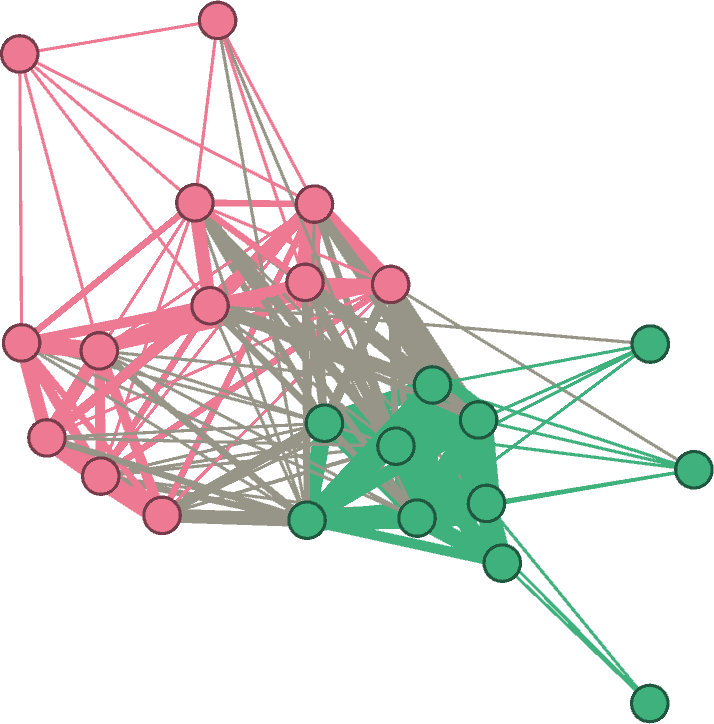
\includegraphics[width=7.5cm]{img/grafos/1994a.png}}
    \qquad
    \subfigure[fig-1994b][Espectro político dos partidos]{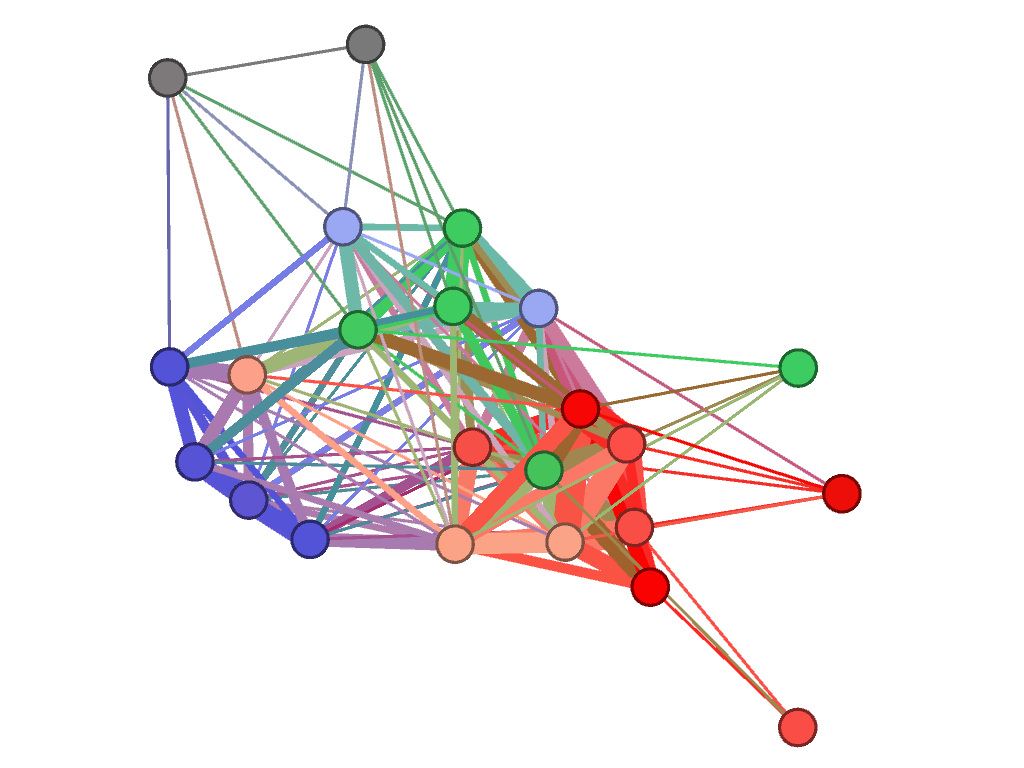
\includegraphics[width=7.5cm]{img/grafos/1994c.png}}

    \caption{1994: Comunidades e espectro político}
\end{figure}

- o grafo é conexo, ou seja, todos os partidos fizeram parte de coligações em pelo menos um estado brasileiro neste ano
- a divisão de esquerda e direita é bem evidente
- os partidos menores com que não conseguimos classificar ficaram nas bordas da componente gigante, indicando que possuem grau menor e consequentemente fizeram menos alianças

\subsection{1998}
\label{resultados__grafos--1998}

\begin{figure}[H]
\center
    \subfigure[fig-1998][Comunidades identificadas]{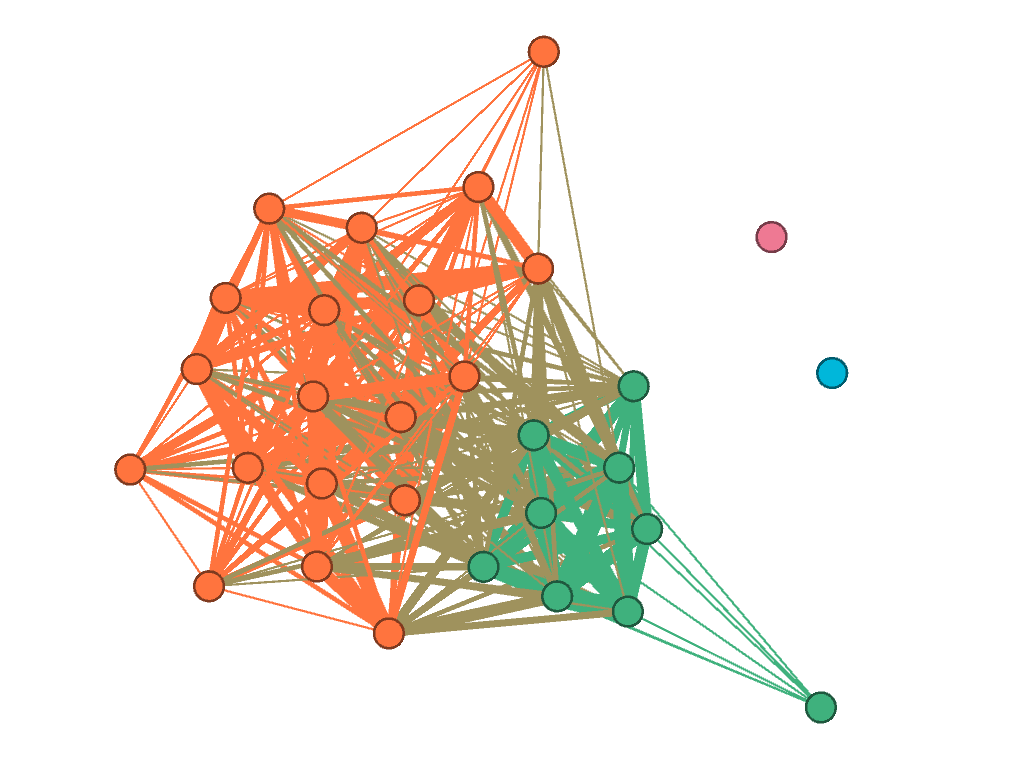
\includegraphics[width=7.5cm]{img/grafos/1998a.png}}
    \qquad
    \subfigure[fig-1998b][Espectro político dos partidos]{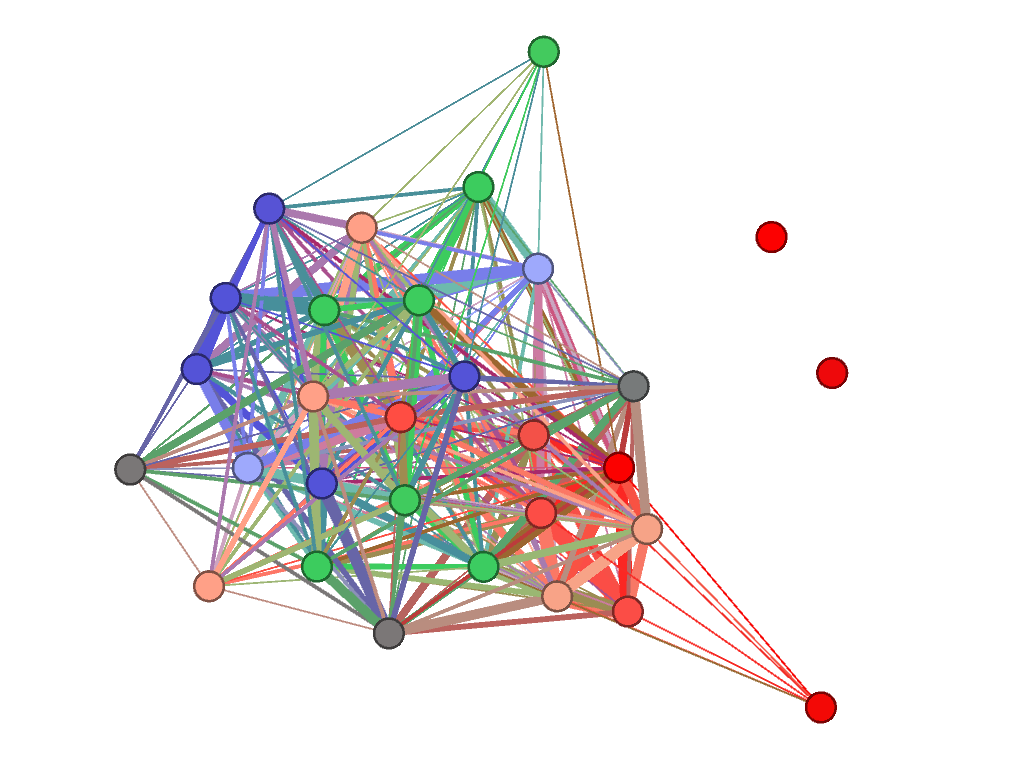
\includegraphics[width=7.5cm]{img/grafos/1998c.png}}

    \caption{comentario}
\end{figure}

\subsection{2002}
\label{resultados__grafos--2002}

\begin{figure}[H]
\center
    \subfigure[fig-2002][Comunidades identificadas]{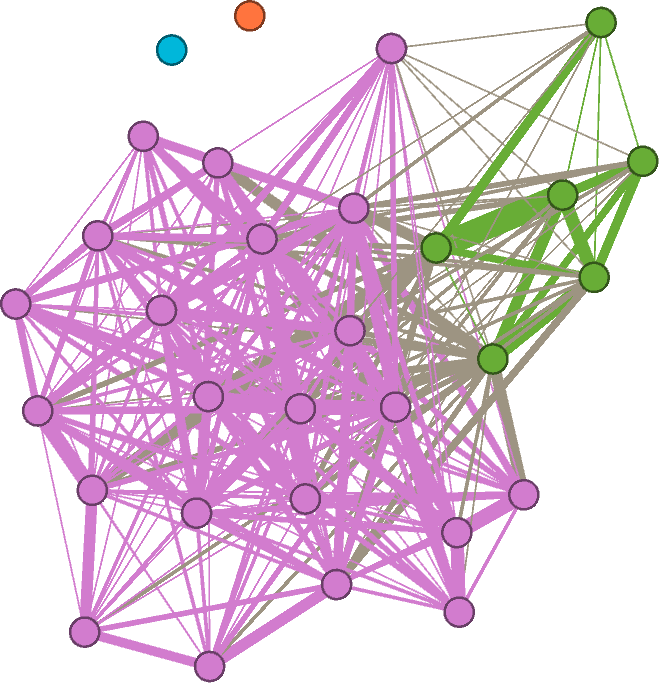
\includegraphics[width=7.5cm]{img/grafos/2002a.png}}
    \qquad
    \subfigure[fig-2002b][Espectro político dos partidos]{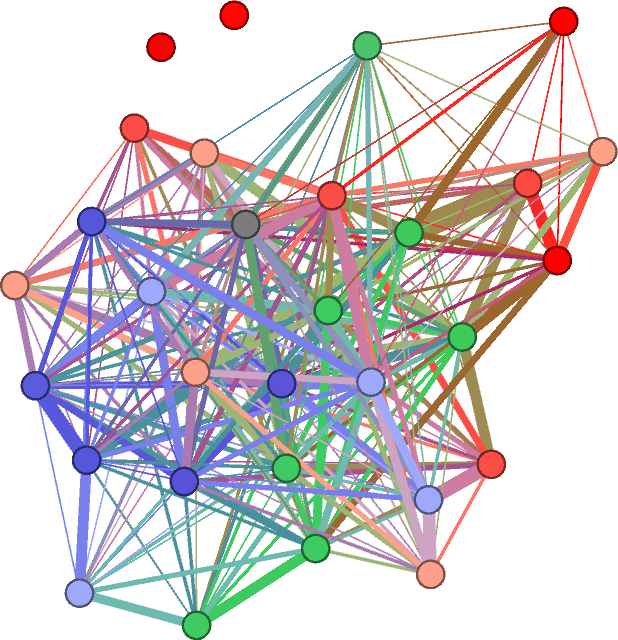
\includegraphics[width=7.5cm]{img/grafos/2002c.png}}

    \caption{comentario}
\end{figure}

\subsection{2006}
\label{resultados__grafos--2006}

\begin{figure}[H]
\center
    \subfigure[fig-2006][Comunidades identificadas]{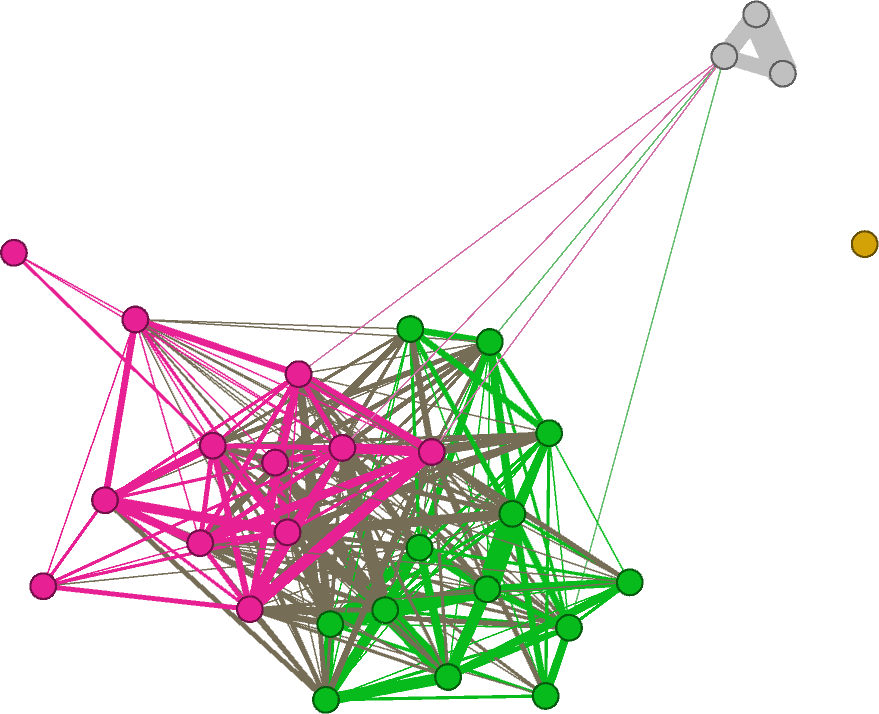
\includegraphics[width=7.5cm]{img/grafos/2006a.png}}
    \qquad
    \subfigure[fig-2006b][Espectro político dos partidos]{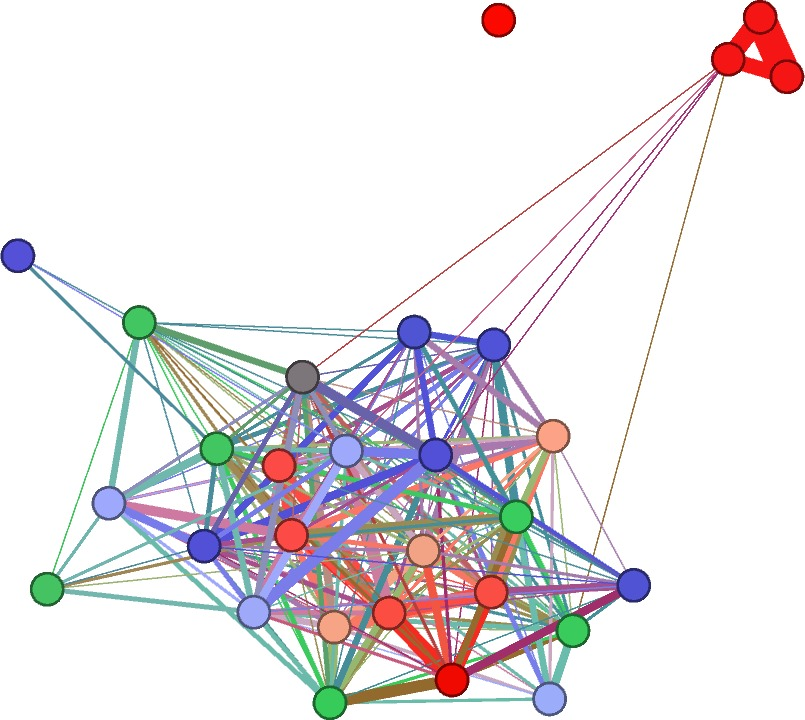
\includegraphics[width=7.5cm]{img/grafos/2006c.png}}

    \caption{comentario}
\end{figure}


\subsection{2010}
\label{resultados__grafos--2010}

\begin{figure}[H]
\center
    \subfigure[fig-2010][Comunidades identificadas]{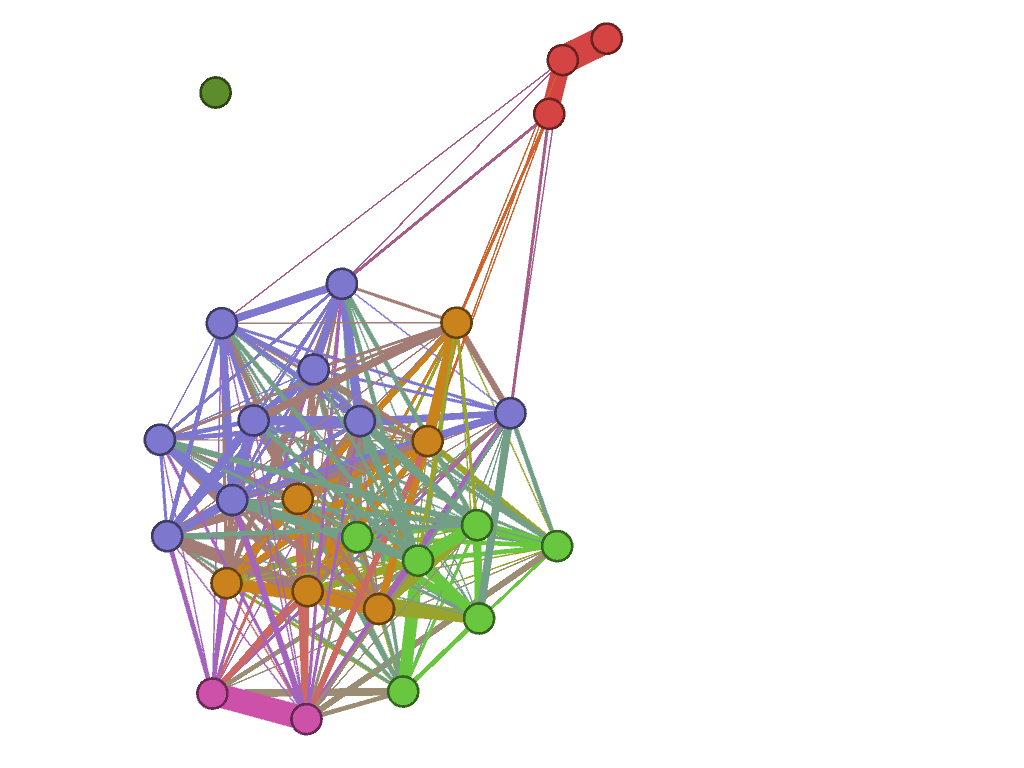
\includegraphics[width=7.5cm]{img/grafos/2010a.png}}
    \qquad
    \subfigure[fig-2010b][Espectro político dos partidos]{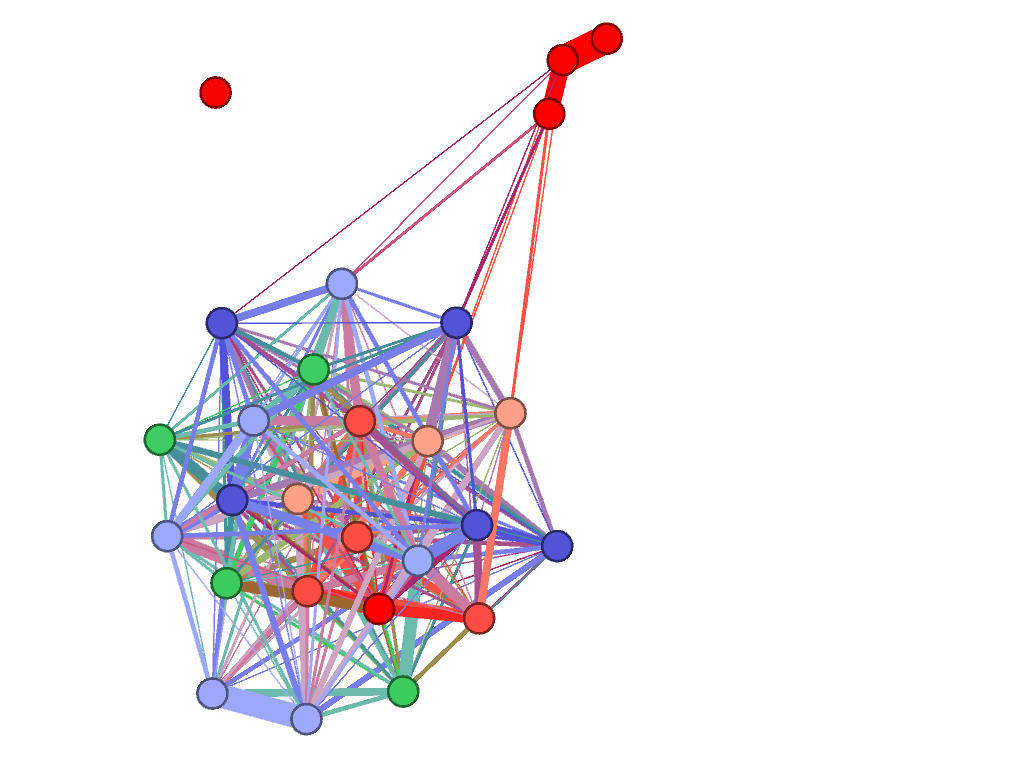
\includegraphics[width=7.5cm]{img/grafos/2010c.png}}

    \caption{comentario}
\end{figure}

\subsection{2014}
\label{resultados__grafos--2014}

\begin{figure}[H]
\center
    \subfigure[fig-2014][Comunidades identificadas]{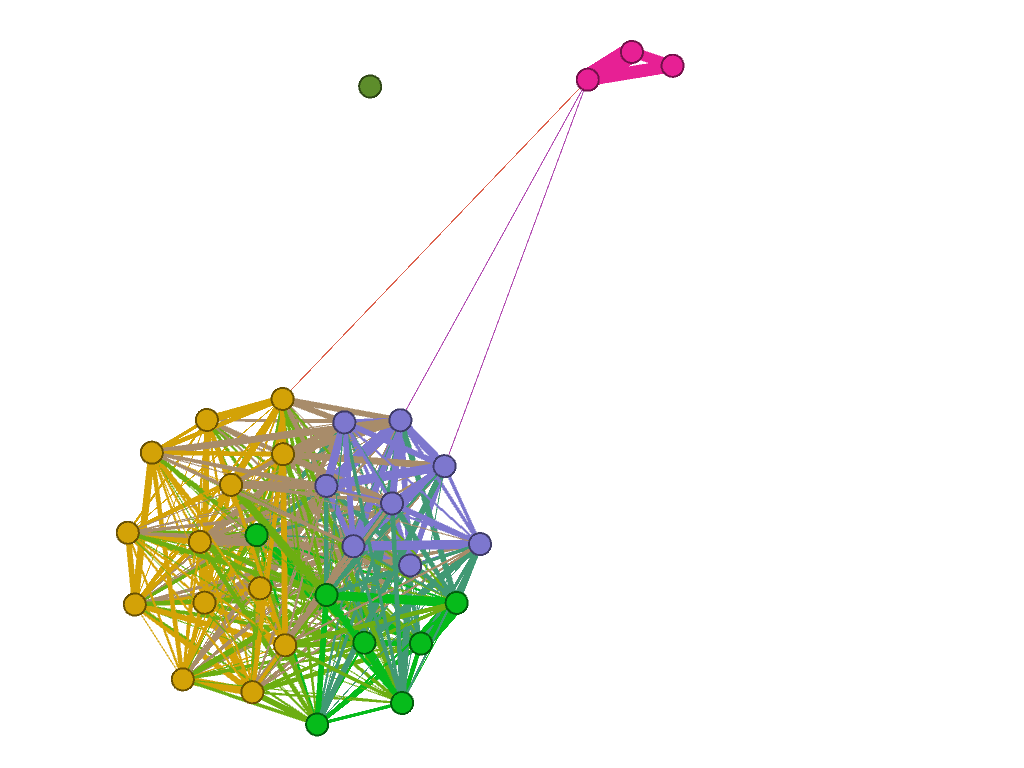
\includegraphics[width=7.5cm]{img/grafos/2014a.png}}
    \qquad
    \subfigure[fig-2014b][Espectro político dos partidos]{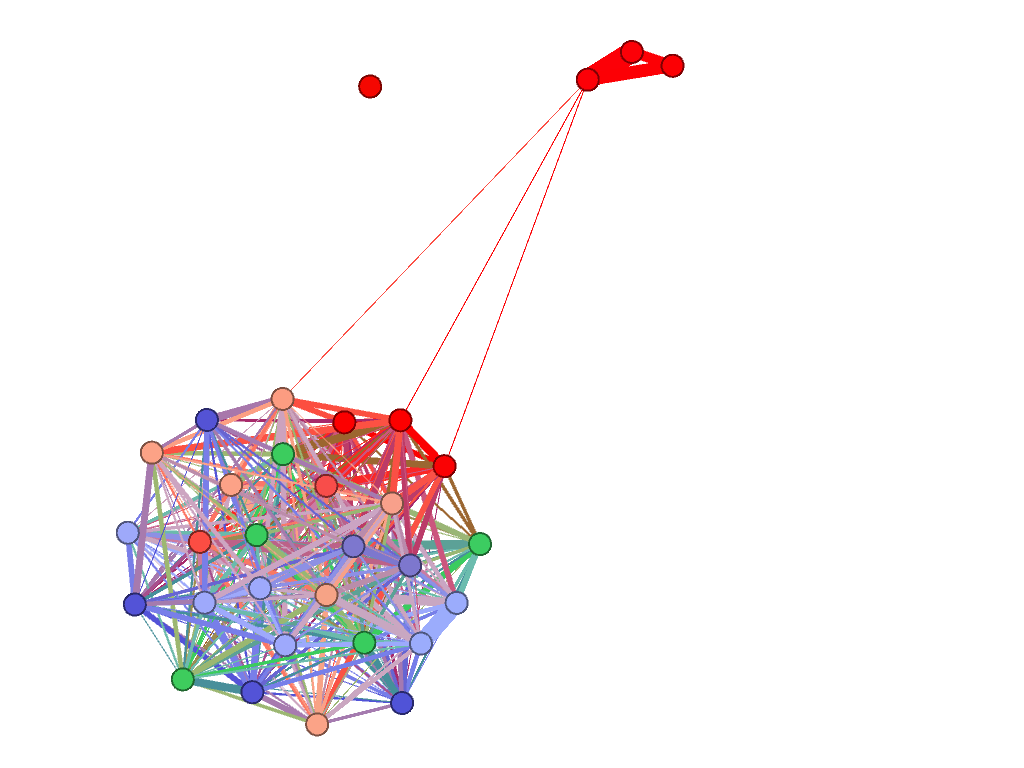
\includegraphics[width=7.5cm]{img/grafos/2014c.png}}

    \caption{comentario}
\end{figure}


%%%%%%%%%%%%%%%%%%%%%%%%%%%%%%%%%%%%%%%%%%%%%%%%%%%%%%%%%%%
\section{\texorpdfstring{\MakeUppercase{Conclusão geral}}{}}
\label{resultados__conclusao-geral}

Conclusão geral
